\documentclass[12pt,a4paper]{article}
%    \usepackage{xeCJK}
\usepackage{amsmath}
\usepackage{graphicx}
    \title{Report}
    \author{An Optical Ray-tracer}
\begin{document}
\maketitle

Optical ray tracing is a very important technique both in optical area and computer graphics area. In optical engineering industry it can help designing and evaluating an optical system, and in computer graphics industry it is important for mimicking the lighting and shadowing effect in real world. This project focuses in simulating paraxial optical system. A object-oriented python script is completed, where scientific calculation and visualization package Numpy and Matplotlib were implemented.
\section{Procedure Description}
The process for a simulation can be implemented step by step as following:
\begin{itemize}
\item Build a model of the optical system concerned, by generating several spherical surface. plane can also be considered a sphere whose curvature equals to zero.
\item Estimate the focus of the optical system by using a 'testray' which is very close to the optical axis. If no real image can be generated (the image might be virtual, but will not be considered in this script.) wrong message will appear and nothing will return.
\item Place an output plane at the focus calculated.
\item Generate a bundle of parallel light rays and run the main simulation procedure.
Store the result and visualize it, calculate the RMS deviation of the ray position from the optical axis.
\end{itemize}

Snell's law is used to compute where a emitted light ray will go after hit on an optical element surface in the main simulation procedure, and reflection is ignored for simplification. For a single element, the process including:
\begin{itemize}
\item Capture the direction of the light ray concerned.
\item Compute the intercept of the input light ray on the surface;
\item Compute the unit normal vector on that intercept point;
\item Compute the output direction of that input light by implementing 3D Snell's law. The formula for the direction of an output ray in 3D goes like this:
$$\hat{s_2}=\frac{n_1}{n_2}[\hat{N}\times(-\hat{N}\times\hat{s_1})]-\hat{N}\sqrt{1-(\frac{n_1}{n_2})^2|\hat{N}\times\hat{s_1}|^2}$$
Here $n_1$ and $n_2$ are refraction index in two mediums outside and inside of the surface respectively, vector $\hat{N}$ stands for unit normal vector on the surface, and $s_1$ is the input ray's direction.
\end{itemize}
\section{Result}
In this simulation program, two models, the simple spherical surface model and the planoconvex lens model, which are described in the project guidelines, are built-in. And two different modes for simulation, random rays and polar symmetrical rays, can be implemented to initialize light rays. Here only symmetrical rays and planoconvex lens model are considered.

The visualization result shows how light rays propagate and how the spots distribute at both the initial position and on the output plane. The result when the spherical surface faces the light is given by the pictures below:\\
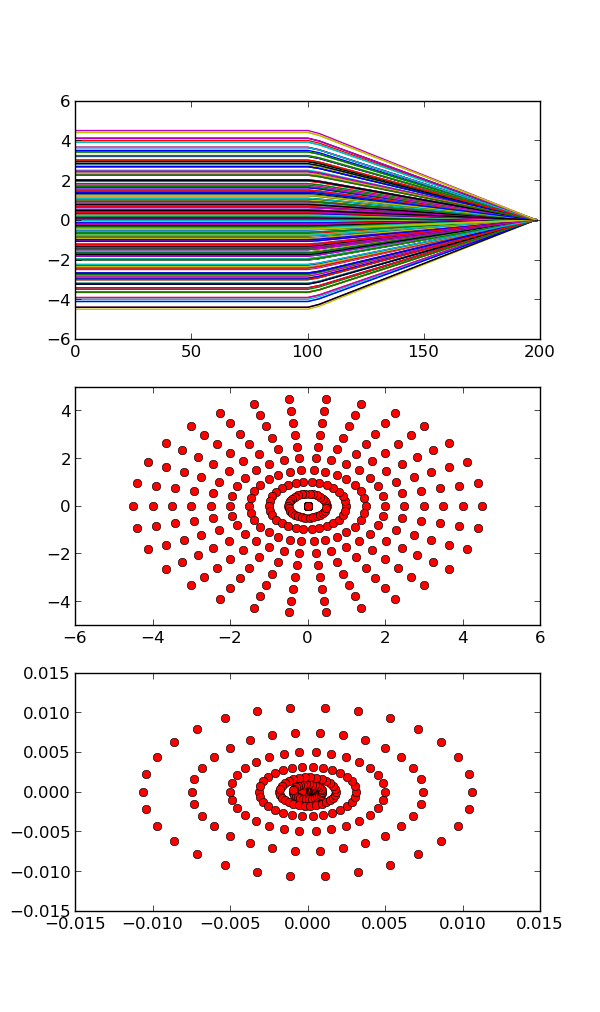
\includegraphics[width=10cm]{figure_1.png} \\
Here the initial bundle of light rays has a diameter of 10mm. Obviously, the closer the input light rays are, the better it is focused. It's RMS deviation from optical axis is also calculated, which is 4563.3nm. This number also has a physical meaning of the radius of geometrical focus of this system. Comparing it to its wave length(588nm), the wave length is way smaller than the diameter of geometrical focus of this system.

The plot for the situation when the plane surface faces the light is similar, however the RMS deviation is totally different, which is 18159.5nm, which is much greater than the situation when spherical surface facing the light. From this result we can easily make an conclusion, that the lens performs better when the spherical surface facing the light rays.


\end{document}